\documentclass[12pt,reqno]{amsart}
\usepackage{array,arydshln}
\usepackage{amsfonts,amssymb,amsmath,amsthm,
            amssymb,amsopn,amsxtra,amstext,amsbsy}
\usepackage{subfig} % To add subfigures
\usepackage[makeroom]{cancel}
%%\usepackage{graphicx}
\usepackage{epsfig}
\usepackage{array}
\usepackage{url}
\usepackage[spanish]{babel}
\usepackage{color}
%\usepackage{float}
\usepackage{savesym}
\savesymbol{AND}
\usepackage{algorithm}
\usepackage{algorithmic}
\usepackage{enumerate}
\newtheorem*{myteo}{Teorema}
\newtheorem*{mydef}{Definici\'on}
\renewcommand{\algorithmicrequire}{\textbf{Input:}}
\renewcommand{\algorithmicensure}{\textbf{Output:}}
\def\R{{\mathbb R }}
\def\N{{\mathbb N }}
\voffset=-10mm
\oddsidemargin=0pt 
\evensidemargin=0pt
\topmargin=-10mm
\headsep=10mm
\headheight=18pt 
\footskip=30pt
\topskip=0mm
\textwidth 167mm
\textheight=230mm
\parindent=5mm 
\marginparsep=3mm
\marginparwidth=19mm
%\renewcommand{\baselinestretch}{2} %double spacing
\vfuzz2pt % Don't report over-full v-boxes if over-edge is small
\hfuzz6pt % Don't report over-full h-boxes if over-edge is small

%% MYREMARK ENVIRONMENT %%%%%%%%%%%
\newenvironment{mycolor}{\color{red}}{}
\newcounter{myremarkcount}
\setcounter{myremarkcount}{0}
\newsavebox{\myremarkbox}
\newenvironment{myremark}
{% This is the begin code
\medskip
\begin{flushright}
\begin{lrbox}{\myremarkbox}%
\begin{minipage}[t]{0.9\linewidth}
\stepcounter{myremarkcount}
\footnotesize
\begin{mycolor}
{\bf Remark \arabic{myremarkcount}.}
\begin{it}
}
{% This is the end code
\end{it}
\end{mycolor}
\end{minipage}
\end{lrbox}
\fbox{\usebox{\myremarkbox}}
\end{flushright}

\bigskip}


\addtolength{\itemsep}{1.5\baselineskip}

\title{An Online  Vector error correction model for forecasting exchange rates}
\author[P. Arce]{Paola Arce}
\address[Paola Arce]{Departamento de Inform\'atica, UTFSM}
\email{paola.arce@usm.cl}
\author[W. Kristjanpoller]{Werner Kristjanpoller} 
\address[Werner Kristjanpoller]{Departamento de Industrias, UTFSM}
\email{werner.kristjanpoller@usm.cl}
\author[L. Salinas]{Luis Salinas}
\address[Luis Salinas]{Departamento de Inform\'atica, UTFSM \and CCTVal, UTFSM}
\email{luis.salinas@usm.cl}


\begin{document}

\maketitle

\begin{abstract}
Foreign exchange rates have been studied as a set of economic
variables whose relationship is said to be cointegrated. When
cointegration exists there are several models which attempt to predict
their future behaviour using historical information. In particular,
vector error correction (VEC) model is an econometric time series
framework widely used to characterize the joint dynamic behaviour of a
set of cointegrated variables. VEC is a particular case of the vector
autoregression (VAR) model that models a set of any variables
capturing linear interdependence among them.  As well as VAR and VEC
model parameters are obtained using the ordinary least squares (OLS)
method.  Even though OLS is extensively used, it has over-fitting
issues and is computationally expensive.  Due to the amount of new
information available in foreign exchange markets, the using of VAR
and VEC models is not suitable in online contexts.  In this article we
present a new model able to obtain VEC parameters faster which are
less adjusted to the data. Our model can be used in online contexts
due to its reduced the response time and because it considers a
portion of the historical data.
\end{abstract} 


\section{Introduction}
The learning from examples problem is an ill-posed problem which
admits an infinite number of solutions.  In order to restrict the
space of admissible solutions, the regression problem is usually
formulated in terms of regularization theory~\cite{girosiETal1995} as
an optimization problem, which minimizes the functional: 

\begin{equation}
\label{eq:problem} 
J(\mathbf{w}) = \sum_{t=1}^m (y_t - f(\mathbf{x}_t))^2 + \gamma R(\mathbf{w})
, \qquad f \in \mathcal{H} \, ,
\end{equation}

\noindent where $m$ is the number of samples $(\mathbf{x}_t ,y_t)$ with
$\mathbf{x}_t \in \R^l$, $l$ correspond to the number of features, $y_t
\in \R$ is the target, $R(\mathbf{w}) = ||w||^2$ where $||.||^2_K$ is a norm in a
{\em reproducing kernel hilbert space} $\mathcal{H}$ defined by the
positive definite form $K$, and $\gamma$ is a regularization
parameter~\cite{evgeniouETal2000}.
%Qué norma debe usarse? falta definir K
When the hypothesis space is reduced, the risk of overfitting the training data
decreases and therefore leading to better generalization capability. 
%aclarar porqué se reduce el espacio de hipótesis
{\em Ridge regression} (RR) is a batch method generally used to solve this
problem, which is a generalization of least squares method (LS). 

%RR is a batch method and it is not used in an online context mainly because
%it uses large amount of data and the number of operations increases
%with data size.

However, online algorithms are more attractive than batch algorithms because
their simplicity and ability to manage large data sets, this is why
they are popular in financial applications.

There are several popular online methods such as
perceptron~\cite{rosenblatt58},
passive-aggressive~\cite{crammerETall2006}, stochastic gradient
descent~\cite{zhang2004}, aggregating algorithm~\cite{vovk2001} and
the second order perceptron~\cite{cesa-bianchi2005}.
In~\cite{cesa-bianchi2006} it is provided an in-deph analysis of
online learning.

The {\em aggregating algorithm for regression} (AAR) method formulates
a recursive formulation of RR in an online way. AAR
consider all data to make a prediction, but in highly variant
scenarios the old data could be useless.

In this paper, we propose an online method based on the idea presented
by~\cite{vovk2001} considering in our case a single sliding window of
the most recent data. This proposal also reduces the number of
operations at every step of the algorithm by expressing the inverse
matrix in an iterative form. Our algorithm is later tested with
financial data from stock market.




\section{Vector autorregresive models}\label{sec:varvec}

VAR as well as VEC are autorregresive models which describe the joint
behaviour of a set variables. Since VEC is a special case of VAR
model, we will formulate the VAR model first and then show how it is
related to the VEC model. 


VAR($p$) model is a general framework to describe
the behaviour of a set of $l$ endogenous variables as a linear
combination of their last $p$ values. These $l$ variables at time $t$
are represented by the vector $\mathbf{y}_t$ as follows:

\begin{equation}
\label{eq:variables}
\mathbf{y}_t = 
\begin{bmatrix} y_{1,t} \\
y_{2,t} \\
\vdots \\
y_{l,t}
\end{bmatrix}
\end{equation}
\noindent where $y_{j,t}$ corresponds to the time series $j$ evaluated at
time $t$.

The VAR(p) model describes the behaviour of a dependent variable in terms
of its own lagged values and the lags of the others variables in the
system. The model with $p$ lags is formulated as the following:

\begin{equation}
\label{eq:var}
 \mathbf{y}_t = \phi_1 \mathbf{y}_{t-1}  + \dots +   \phi_p\mathbf{y}_{t-p}
+ \mathbf{c} + \mathbf{\epsilon}_t, \qquad t=p+1, \dots, N
\end{equation}

\noindent where ${\phi_1,\dots,\phi_p}$ are $l \times l$ 
matrices of real coefficients, $\mathbf{\epsilon}_{p+1},\dots,\mathbf{\epsilon}_N$ are
error terms, $\mathbf{c}$ is a constant vector and $N$ is the total number of
samples.

The VAR matrix form is the following:

\begin{equation}
 \label{eq:varmatrix}
               \underbrace{ \begin{bmatrix}
               \quad \\
               \mathbf{y}_{p+1} &
               \mathbf{y}_{p+2} &
               \dots & 
               \mathbf{y}_N \\
               \quad
               \end{bmatrix}}_{\substack{ \mathbf{B}^\top\\l \times (N-p)}}   
= 
                \underbrace{\left[ 
                \begin{array}{ccccc}
                \quad & \quad & \quad & \quad & \quad \\
                \phi_1  & \phi_2 & \cdots & \phi_p & \mathbf{c} \\  
                \quad &\quad & \quad & \quad & \quad
               \end{array} 
               \right]}_{\substack{ \mathbf{X}^\top\\ l \times (l \times p + 1 )}}
\underbrace{\begin{bmatrix}
   \mathbf{y}_{p}  & \mathbf{y}_{p+1} & \dots    & \mathbf{y}_{N-1}\\
   \mathbf{y}_{p-1}  & \mathbf{y}_{p} & \dots    & \mathbf{y}_{N-2}\\
   \vdots        & \vdots   & \ddots   & \vdots\\
   \mathbf{y}_{1} & \mathbf{y}_{2}   & \dots    & \mathbf{y}_{N-p}\\
   1 & 1   & \dots    & 1 
   \end{bmatrix}}_{\substack{ \mathbf{A}^\top\\ (l\times p +1 )\times (N-p)}}
+
\underbrace{\begin{bmatrix}
                \quad \\
              \mathbf{\epsilon}_{p+1}  & 
              \mathbf{\epsilon}_{p+2}  & 
              \dots                & 
              \mathbf{\epsilon}_N \\
              \quad
             \end{bmatrix}}_{\substack{\mathbf{E}^\top\\l \times (N-p) }} 
\end{equation}

\noindent which can be solve using ordinary least squares estimation.


\section{Integration and Cointegration}

A time series $\mathbf{y}$ is called integrated of order $d$ if after
differencing the variable $d$ times, we get a I(0) variable (stationary
process), i.e:
\[
(1-L)^d \mathbf{y} \sim \text{I(0)}
\]
\noindent where I(0) is a stationary time series and $L$ is the lag operator, i.e,
\[
(1-L)\mathbf{y} = \Delta \mathbf{y}
\]
\noindent where $\Delta \mathbf{y}(t) = \mathbf{y}(t)  -\mathbf{y}(t-1) \quad \forall t $.


Let $\mathbf{y}_t = \{\mathbf{y}^1, \dots, \mathbf{y}^l\}$ be a set of $l$ stationary time
series I(1) which are said to be cointegrated if a vector
$\beta=[\beta(1),\dots,\beta(l)]^\top \in \mathbb{R}^l$  exists such that the time series,

\begin{equation}
 \mathbf{Z}_t:= \beta^\top \mathbf{y}_t = \beta(1) \mathbf{y}^1 + \dots + \beta(l) \mathbf{y}^l \sim
 \text{I(0)}
\end{equation}

In words, a set of I(1) variables is said to be cointegrated if
exists a linear combination of them which is I(0).

\subsection{Stationary Time Series}

A strictly stationary times series is one for which the probabilistic behavior
of every collection of values $\{y_{t_1},y_{t_2},\dots,y_{t_L}\}$ is identical
to that of the time shifted set, more precisely: \[ P\{y_{t_1} \leq
c_1,\dots,y_{t_L} \leq c_L\} = P\{y_{t_1+h} \leq c_1,\dots,y_{t_L+h}
\leq c_L\}
\quad \forall L \in \mathbb{N}, \forall h \in \mathbb{Z}\] \noindent where
$c_1,\dots,c_L$ are constants.

This definition is too strong and difficult to assess it from a single data
set. The weak version of this definition imposes conditions only on the two
first two moments.

A weakly stationary time series is a process which mean, variance and auto
covariance do not change over time:

\begin{eqnarray*}
E(Y_t) &=& \mu  \quad \forall t \in \mathbb{N} \\ E(Y^2_t) &=&
\sigma^2  \quad \forall t \in \mathbb{N} \\
\lambda(s,t)&=&\lambda(s+h,t+h) \quad \forall s,t \in \mathbb{N},
\forall h \in \mathbb{Z}
\end{eqnarray*}

\noindent with $\lambda(s,t) = E[(y_s-\mu)(y_t - \mu)]$.

The following example~\cite{johansen1995} helps to illustrate the meaning
of $\beta$:

\textbf{Example:}

If we have two-dimensional process $\mathbf{X}_t$, $t=1,\dots,T$ by:

\begin{eqnarray*}
\mathbf{X}_{1t} &=& \sum_{i=1}^t \epsilon_{1i} + \epsilon_{2t} \\
\mathbf{X}_{2t} &=& a \sum_{i=1}^t \epsilon_{1i} + \epsilon_{3t} 
\end{eqnarray*}

Since $\mathbf{X}_{1t}$ and $\mathbf{X}_{2t}$ are I(1) processes and there
exist a vector $\beta = [a -1]$ such that:

\[
\beta^\top \mathbf{X}_t = a \mathbf{X}_{1t} -\mathbf{X}_{2t} = 
a\epsilon_{2t} - \epsilon_{3t} \sim \text{I(0)}
\]

then, both processes are said to be cointegrated. If we add a I(0) process
$\mathbf{X}_{3t} = \epsilon_{4t}$  we find that there exists two cointegration
vectors now: $\begin{bmatrix}a &-1& 0\end{bmatrix}$ and $\begin{bmatrix}0
&0&1\end{bmatrix}$ since:

\[
\beta^\top \mathbf{X}_t = 
\begin{bmatrix}
a & -1 & 0 \\
0 & 0 & 1
\end{bmatrix} 
\begin{bmatrix} 
\mathbf{X}_{1t} \\
\mathbf{X}_{2t} \\
\mathbf{X}_{3t}
\end{bmatrix} = 
\begin{bmatrix}
a\epsilon_{2t} - \epsilon_{3t} \\
\epsilon_{4t}
\end{bmatrix}
\]

This example shows how cointegration vectors describes the stable relations
between the processes by linear relations that are more stationary than the
original process.

\section{VEC model}

A VEC model is a special form of a VAR model for I(1) variables that
are also cointegrated. The VEC model is obtained by replacing the form
$\Delta \mathbf{y}_t = \mathbf{y}_t - \mathbf{y}_{t-1}$ in equation
(\ref{eq:var}). The VEC model is expressed in terms of differences,
has an error correction term and it has the following form:

\begin{equation}
 \label{eq:vec}
 \Delta \mathbf{y}_t = 
 \underbrace{ \Omega\mathbf{y}_{t-1}}_\text{Error correction term} + 
 \sum_{i=1}^{p-1}
\phi_i^* \Delta \mathbf{y}_{t-i}  + \mathbf{c} + \mathbf{\epsilon}_t \quad ,
\end{equation}

\noindent where coefficients matrices $\Omega$ and $\phi_i^*$ are
function of matrices $\phi_i$ (shown in equation (\ref{eq:var})) as follows:

\begin{eqnarray*}
\phi_i^* &: =& -\sum_{j=i+1}^{p} \phi_j \\
\Omega &: =& -(\mathbb{I}-\phi_1-\dots-\phi_p) 
\end{eqnarray*}

The matrix $\Omega$ has the following properties:
\begin{itemize}
\item If $\Omega = 0$ there is no cointegration
\item If $rank(\Omega)=l$ i.e full rank, then the time series are not
I(1) but stationary
\item If $rank(\Omega)=r,\quad 0 < r < l$ then, there is cointegration
and the matrix $\Omega$ can be expressed as $\Omega =
\alpha \beta^\top$, where $\alpha$ and $\beta$ are $(l \times r)$
matrices and $rank(\alpha)=rank(\beta)=r$.

The columns of $\beta$ contains the cointegration vectors and the rows of
$\alpha$ correspond with the adjusted vectors. $\beta$ is obtained by Johansen
procedure~\cite{johansen1988} whereas $\alpha$ has to be determined as a
variable in the VEC model.

It is worth noticing that the factorization of the matrix $\Omega$ is not unique since for any
$r \times r$ nonsingular matrix $H$ we have:

\begin{eqnarray*}
\alpha \beta^\top &=& \alpha \mathbf{HH^{-1}} \beta^\top\\
&=&(\alpha\mathbf{H})(\beta(\mathbf{H}^{-1})^\top)^\top \\
&=& \alpha^*(\beta^*)^\top
\end{eqnarray*}

\noindent whith $\alpha^* = \alpha\mathbf{H}$ and $\beta^* =
\beta(\mathbf{H}^{-1})^\top$.

Therefore, to obtain unique values, further restrictions on the model
are required.

\end{itemize}
%Johansen  procedure also gives a set of
%eigenvalues ordered in a descending way which do not correspond to
%$\alpha$ but the number of eigenvalues larger than zero determine the rank
%of $\beta$, i.e the number of cointegration relations. 

If cointegration exists, then equation (\ref{eq:vec}) can be written as follows:


\begin{equation}
 \label{eq:vecfull}
 \Delta \mathbf{y}_t = \alpha \beta^\top\mathbf{y}_{t-1} 
 + \sum_{i=1}^{p-1} \phi_i^*\Delta
\mathbf{y}_{t-i}  + \mathbf{c} + \mathbf{\epsilon}_t \quad ,
\end{equation}

\noindent which is a VAR model but for time series differences.

The matricial form of the VEC model is the following:

\begin{equation} \label{eq:vecmatrix}
\underbrace{
               \begin{bmatrix}
               \quad\\
                \mathbf{\Delta y}_{p+1} & 
                \dots &
                \mathbf{\Delta y}_N \\
                \quad
               \end{bmatrix}
               }_{\substack{\mathbf{B}^\top\\ l \times (N-p) }} =
   \underbrace{
    \begin{bmatrix}
     \quad \\
     \alpha & \phi_1^* & \cdots & \phi_{p-1}^* & \mathbf{c} \\  
     \quad
     \end{bmatrix} 
     }_{\substack{ \mathbf{X}^\top\\ l \times (l\times p +1)}}
\underbrace{\begin{bmatrix} 
   \beta^\top \mathbf{y}_{p} & 
   \cdots & \beta^\top \mathbf{y}_{N-1} \\
   \mathbf{\Delta y}_p  & \cdots 
   & \mathbf{\Delta y}_{N-1} \\ 
   \vdots  & \ddots & \vdots \\
   \mathbf{\Delta y}_2  & \cdots 
   & \mathbf{\Delta y}_{N-p+1} \\
   1 & \cdots & 1 
   \end{bmatrix}}_{\substack{\mathbf{A}^\top \\ (l \times p +1) \times (N-p) }}
+
\underbrace{\begin{bmatrix}
              \quad \\
              \mathbf{\epsilon}_{p+1} &
              \dots &
              \quad &\mathbf{\epsilon}_N \\ \quad
             \end{bmatrix}}_{\substack{\mathbf{E}^\top\\ l \times (N-p) }} 
\end{equation}

VAR and VEC model parameters shown in equations (\ref{eq:varmatrix}) and
(\ref{eq:vecmatrix}) can be solve using standard regression techniques, such as
ordinary least squares (OLS). However, matrix $\mathbf{A}$ is usually
rank-deficient and OLS solution could not be found. Ridge regression method (RR)
is commonly used instead of OLS when matrices are ill-conditioned or
rank-deficient since it has improved generalization capabilities.


\section{Regression problems} \label{sec:OLS}

VAR as also VEC model parameters requires solving the following
multiple regression problem:

\begin{equation}
\label{eq:regproblem}
\underset{m \times n}{\mathbf{A}} \enskip \underset{n \times
l}{\mathbf{\phi}} = \underset{m \times l}{\mathbf{B}}
\end{equation}

In the case matrix $\mathbf{X}$ is non singular, its solution is
straight forward:

\begin{equation}
\label{OLSsolution}
    \mathbf{X}=\mathbf{X}^{-1}\mathbf{B}
\end{equation}

\subsection{Ordinary least squares}
When $\mathbf{X}$ is singular, solution to
equation~(\ref{eq:regproblem}) is given by the ordinary least squares
(OLS) method. OLS consists of minimizing the sum of squared errors or
equivalently minimizing the following expression:

\begin{equation}
\label{eq:regressionproblem}
\underset{\mathbf{X}}{\text{min}} \quad \| \mathbf{X}\mathbf{\mathbf{X}} - \mathbf{B} \|_2^2
\end{equation}

\noindent which solution $\hat{\mathbf{X}}$ is well-known:

\begin{equation}
\label{eq:MP}
\hat{\mathbf{X}}=\mathbf{X}^+\mathbf{B}
\end{equation}

\noindent where $\mathbf{X}^+$ is the Moore-Penrose pseudo-inverse
which can be written as follows: 

\begin{equation}
\label{eq:pseudoinverse}
\mathbf{X}^+= (\mathbf{X}^\top \mathbf{X})^{-1}\mathbf{X}^\top \, .
\end{equation}

However, when $\mathbf{X}$ is not full rank, i.e
$rank(\mathbf{X})=k <  n \leq m$, $\mathbf{X}^\top \mathbf{X}$ is
always singular and equation~(\ref{eq:pseudoinverse}) cannot be used.
More generally, the pseudo-inverse is best computed using the compact
singular value decomposition (SVD) of $\mathbf{X}$:

\begin{equation}
    \label{eq:compactsvd}
    \underset{m \times n}{\mathbf{X}}=
    \underset{m \times k}{\mathbf{U_1}} \enskip
    \underset{k \times k}{\mathbf{\Sigma_1}} \enskip
    \underset{k \times n}{\mathbf{V_1}^\top}
\end{equation}

\noindent as follows

\begin{equation}
\label{eq:pseudoinversesvd}
\mathbf{X}^+ = \mathbf{V_1\Sigma_1^{-1}U_1^\top}
\end{equation}




\textbf{Demo}\quad

Since the problem shown in equation~(\ref{eq:regproblem}) has not
solution, the minimum norm given by equation~(\ref{OLSsolution}) is
obtained by solving the equivalent problem:

\begin{equation*}
\label{eq:proyectorsol}
\mathbf{X \hat{\phi} = PB} 
\end{equation*}

\noindent where $\mathbf{P=U_1 U_1^\top}$ is the projection onto the
Col($\mathbf{X}$). 

Since $\mathbf{V} = [\underset{(n \times k)}{\mathbf{V_1}} |
\underset{(n \times k)}{\mathbf{V_2}}]$ and $\mathbf{V_1^\top V_2 =
0}$ we can express $\mathbf{\hat{\phi}} = \mathbf{V_1 x_1 + V_2 x_2}$
with $\mathbf{x_2=0}$ because $\mathbf{\hat{\phi}}$ lives in the
$\text{Row}(\mathbf{X})$ given by $\mathbf{V_1}$, so we have:

\begin{eqnarray*}
\mathbf{X \hat{\phi}} &=& \mathbf{PB} \\
\mathbf{U_1 \Sigma_1 V_1^\top \hat{\phi}} &=& \mathbf{U_1 U_1^\top B} \\
\mathbf{ V_1^\top \hat{\phi}} &=&  \mathbf{\Sigma_1^{-1} U_1^\top B} \\ 
\mathbf{ V_1^\top V_1 x_1} &=& \mathbf{\Sigma_1^{-1}
U_1^\top B} \\
\mathbf{x_1}&=& \mathbf{\Sigma_1^{-1} U_1^\top B}
\end{eqnarray*}

\noindent from this result we can obtain $\mathbf{\hat{\phi}}$ and
therefore the pseudo-inverse expression:

\begin{eqnarray*}
\mathbf{\hat{\phi}} &=& \mathbf{V_1 x_1} \\
                &=& \mathbf{V_1 \Sigma_1^{-1} U_1^\top B} \\
\mathbf{X^+} &=& \mathbf{V_1 \Sigma_1^{-1} U_1^\top} \, .
\end{eqnarray*}




\section{Ridge Regression}
\subsection{Regression problems}
The objective of regression problems is to find a function $f$ which
explains the relation between an input $\mathbf{x}_t \in \R^l$, and an
output $y_t \in \R$ such that: $y_t=f(\mathbf{x}_t) + \epsilon_t$ for
a set of $m$ data points $\{( \mathbf{x}_t,y_t)\}_{t=1}^m$.  If the
relationship between $y_t$ and $\mathbf{x}_t$ is thought to
be linear, $f$ can be written as:

\begin{equation*}
f(\mathbf{x}_t)=\mathbf{w}^\intercal \mathbf{x}_t=\sum_{i=1}^l
w(i)x_t(i) \, ,
\end{equation*}

\noindent where $\mathbf{w}$ is a  weight vector determined in a training phase.

The least squares method is a well known way to solve a regression
problem. This method consists of minimizing the sum of squared error:


\begin{equation}
\label{eq:problem2}
 J(\mathbf{w}) = \sum_{t=1}^m (f(\mathbf{x}_t)-y_t)^2 = \sum_{t=1}^m
 (\mathbf{w}^\intercal {\bf x}_t-y_t)^2 \, ,
\end{equation}

\noindent which is equivalent to minimize $J(\mathbf{w})$ with $\gamma = 0$ in
equation~(\ref{eq:problem}). 
Expressed in matrix form this amounts to: %verificar inglés con profe

\begin{equation*}
J(\mathbf{w})=
	\big\|
       \begin{bmatrix}
       x_1(1) & \cdots & x_1(l) \\
       \vdots & \ddots & \vdots \\
       x_m(1) & \cdots & x_m(l)
       \end{bmatrix}
       \begin{bmatrix}
       w(1)\\
       \vdots \\
       w(l) 
       \end{bmatrix}-
       \begin{bmatrix}
        y_1\\
        \vdots \\
        y_m 
        \end{bmatrix}
       \big\|_{L^2}^2
\end{equation*}  

\noindent or a more reduced expression is:

\begin{equation*}
J(\mathbf{w}) = \| \mathbf{X}\mathbf{w} - \mathbf{y} \|_2^2 ,  
\end{equation*}  

\noindent where

\begin{equation*}
\mathbf{X} = \begin{bmatrix} \mathbf{x}_1^\intercal \\ \vdots \\
\mathbf{x}_m^\intercal \end{bmatrix} , \quad
\mathbf{y} = \begin{bmatrix} y_1 \\ \vdots \\ y_m \end{bmatrix} \quad
\text{and}  \quad
\mathbf{w} = \begin{bmatrix} w(1) \\ \vdots \\ w(l) \end{bmatrix}
\end{equation*}
As is well known, the optimal solution $\mathbf{w}_*$ obtained minimizing
equation~(\ref{eq:problem2}) is:

\begin{equation}
\label{eq:MPenrose}
\mathbf{w}_*=(\mathbf{X}^\intercal \mathbf{X})^{-1}\mathbf{X}^\intercal \mathbf{y}
\end{equation}
Thus, when a new input $\mathbf{x}_t$ arrives, the prediction of the target
value $y_t$ is defined as:

\begin{equation*}
f(\mathbf{x}_t)=\mathbf{w}_*^\intercal \mathbf{x}_t \,.
\end{equation*}

\subsection{Ridge Regression}

In order to avoid the singularity of the matrix $\mathbf{X}^\intercal
\mathbf{X}$ in equation~(\ref{eq:MPenrose}), a regularization term is
introduced.  The optimization problem including the regularization
term is shown in equation~(\ref{eq:problem}). 

%\begin{equation*}
%\min_{\mathbf{w}} J(\mathbf{w}), \quad \text{where} \quad J(\mathbf{w}) =
%\sum_{t=1}^m
%(f(\mathbf{x}_t)-y_t)^2  + \gamma R(\mathbf{w}) \, ,
%\end{equation*}
%
%and $\gamma$ is a regularization parameter and term $R(\mathbf{w})$ reduce the
%space of possible solutions simplifying the search in the optimization problem.

When $R(\mathbf{w}) = \| \mathbf{w}\| ^2$, the method is called ridge
regression and the optimal solution $\mathbf{w}_*$ is well known: 

\begin{equation}
\label{eq:optsolRR}
\mathbf{w}_*=(X^\intercal X+\gamma \mathbb{I})^{-1}X^\intercal y \, ,
\end{equation}
Equation~(\ref{eq:optsolRR}) can be also be expressed as:

\begin{eqnarray*}
\mathbf{w}_* =& \displaystyle \big (\sum_{t=1}^m \mathbf{x}_t \mathbf{x}_t  ^\intercal + \gamma
\mathbb{I}\big )^{-1} \sum_{t=1}^m y_t \mathbf{x}_t \\
\mathbf{w}_* =& \mathbf{A}^{-1}\mathbf{b}\, ,
\end{eqnarray*}

\noindent where


\[ 
\mathbf{A}= \sum_{t=1}^m \mathbf{x}_t \mathbf{x}_t  ^\intercal +
\gamma \mathbb{I} 
\qquad \text{and} \qquad 
\mathbf{b}=  \sum_{t=1}^m y_t \mathbf{x}_t 
\, .\]



\begin{algorithm}[H]
\begin{algorithmic}[1]
\REQUIRE $\,$ \\
$\{\mathbf{x}_1,\dots,\mathbf{x}_{m} \}$: $m$ input vectors \\
$\{y_1,\dots,y_{m} \}$: $m$ targets \\
\ENSURE  $\,$ \\
$\{f(\mathbf{x}_1),\dots,f(\mathbf{x}_{m}) \}$: model predictions \\
\STATE Initialize $\mathbf{A}=\gamma \mathbb{I}$
and $\mathbf{b}=0$
\FOR { $t = 1$ to $m$ }
	\STATE read new $\mathbf{x}_t$
	\STATE output prediction $f(\mathbf{x}_t) =  \mathbf{b}^\intercal \mathbf{A}^{-1}\mathbf{x}_t$
   	\STATE $\mathbf{A} = \mathbf{A} + \mathbf{x}_t \mathbf{x}_t^\intercal$
   	\STATE Read new $y_t$
    	\STATE $\mathbf{b} = \mathbf{b} + y_t \mathbf{x}_t$
\ENDFOR

\end{algorithmic}
\caption{Ridge Regression}
\label{alg:RR}
\end{algorithm}

The ridge regression method is shown in algorithm~\ref{alg:RR} where
the prediction value for a new input $\mathbf{x}_{m+1}$ is:

\begin{eqnarray*}
f(\mathbf{x}_{m+1}) =& \mathbf{w}_*^\intercal \mathbf{x}_{m+1} \\
  =& \mathbf{b}^\intercal \mathbf{A}^{-1} \mathbf{x}_{m+1}
\, .
\end{eqnarray*}




%The effect of adding the term $\gamma \mathbb{I}$ to the matrix
%$\mathbf{X}^\intercal \mathbf{X}$ improves 
%its condition number because it increases its diagonal values when $\gamma > 0 $. 
%The matrix $\mathbf{X}^\intercal \mathbf{X}$ is symmetrical
%($(\mathbf{X}^\intercal \mathbf{X})^\intercal = \mathbf{X}^\intercal
%\mathbf{X}$) and is therefore diagonalizable.
%If we now the eigenvalue decomposition of $\mathbf{X}^\intercal \mathbf{X}=\mathbf{VDV}^{-1}$ where the columns of
%$\mathbf{V}$ are its eigenvectors and $\mathbf{D}$ is a diagonal matrix with its eigenvalues,
%then replacing the EVD on equation~(\ref{eq:optsolRR}) we have:
%
%\begin{eqnarray*}
%w_*=&(\mathbf{VDV}^{-1}+ \mathbf{V} \gamma
%\mathbb{I}\mathbf{V}^{-1})^{-1}\mathbf{X}^\intercal \mathbf{Y}\\
%w_*=&(\mathbf{VD}_\gamma \mathbf{V}^{-1})^{-1}\mathbf{X}^\intercal \mathbf{Y} \, ,
%\end{eqnarray*}
%where
%
%\begin{equation*}
%\mathbf{D}_\gamma=
%\begin{bmatrix}
%d_1 + \gamma & \, & \, \\
%\, & d_2 +\gamma & \, \\
%\, & \, & \ddots & \, \\
%\, & \, & \, & d_l +\gamma \, .
%\end{bmatrix}
%\end{equation*}
%where $d_1 \geq d_2 \geq \dots \geq d_l$.
%
%So, the condition number of $\mathbf{A}=\mathbf{X}^\intercal \mathbf{X}+\gamma \mathbb{I}$ is defined as:
%
%\begin{equation*}
%	\kappa = \|\mathbf{A}\| \|\mathbf{A}^{-1}\|
%\end{equation*}
%because $\mathbf{A}$ is simmetrical and therefore non-singular, the condition number can be
%expressed in terms of its eigenvalues:
%
%\begin{eqnarray*}
%\kappa = \frac{\sigma_1}{\sigma_l} \\
%\kappa = \frac{d_1+\gamma}{d_l + \gamma} \,
%\end{eqnarray*}
%which is a better condition number than the problem without regularization
%($\kappa = d_1/d_l$), it means:
%
%\begin{equation*}
%	\frac{d_1+\gamma}{d_l + \gamma} < \frac{d_1}{d_l} \, ,
%\end{equation*}
%for $\gamma > 0$.
%
%
%
%
%
%
%

\section{Efficient computation}

In order to solve OLS in a efficient way, Coleman and
Sun~\cite{coleman+sun2010} presented an iterative algorithm which
uses $\mathbf{X}(\lambda)$ to approximate $\mathbf{X}(0)$.


Using the compact SVD (shown in equation~(\ref{eq:compactsvd}))
$\mathbf{X}(\lambda)$ is expressed as follows:


\begin{eqnarray}
\label{eq:optsolRRsvd}
\mathbf{X}(\lambda) & = & (\mathbf{A}^\top \mathbf{A}+ \lambda
\mathbb{I})^{-1}\mathbf{A}^\top \mathbf{B} \nonumber \\
& = &\mathbf{V}_1(\Sigma_1^2+\lambda \mathbb{I})^{-1}\mathbf{\Sigma_1
U_1^\top B}
\end{eqnarray}

\noindent where is easy to see that $\mathbf{X}(\lambda) \rightarrow
\mathbf{\hat{X}}=\mathbf{V}_1 \mathbf{\Sigma}_1^{-1}\mathbf{U}_1^\top
\mathbf{B}$ as $\lambda \rightarrow 0$. 

The method consists in obtaining $\mathbf{X}(\lambda)$ and then refine
by adding more terms of its Taylor expansion to approximate
$\mathbf{X}(0) = \mathbf{\hat{X}}$. The Taylor expansion about $\lambda_0$ is:

\begin{equation}
\label{eq:taylor}
    \mathbf{X}(\lambda)=\mathbf{X}(\lambda_0) + \sum_{k=1}^\infty
    \mathbf{s}_k(\lambda-\lambda_0)^{k}
\end{equation}


\noindent where $\mathbf{s}_k=\frac{1}{k!}\mathbf{X}(\lambda)^{(k)}$
and $\mathbf{X}(\lambda)^{(k)}$ is obtained by taking differences 
$\frac{\partial}{\partial \lambda}$ of:  

\begin{eqnarray*}
(\mathbf{A}^\top \mathbf{A}+ \lambda\mathbb{I}) \mathbf{X}(\lambda) & = & \mathbf{A}^\top \mathbf{B}\\
(\mathbf{A}^\top \mathbf{A}+ \lambda\mathbb{I}) \mathbf{X}(\lambda)^{(1)} + \mathbf{X}(\lambda)& = & 0 \\
\mathbf{X}(\lambda)^{(1)}  &=& -(\mathbf{A}^\top \mathbf{A}+ \lambda\mathbb{I}) ^{-1} \mathbf{X}(\lambda) \\
\mathbf{X}(\lambda)^{(2)}  &=& -2(\mathbf{A}^\top \mathbf{A}+ \lambda\mathbb{I}) ^{-1} \mathbf{X}(\lambda)^{(1)} \\
& \vdots & \\
\mathbf{X}(\lambda)^{(k)}  &=& -k(\mathbf{A}^\top \mathbf{A}+ \lambda\mathbb{I}) ^{-1} \mathbf{X}(\lambda)^{(k-1)} 
\end{eqnarray*}



\noindent for $\lambda=0$ we have:

\begin{equation}
\label{eq:taylor}
    \mathbf{X}(0)=\mathbf{X}(\lambda_0) + \sum_{k=1}^\infty
     (-1)^k \mathbf{s}_k \lambda_0^k
\end{equation}


\noindent therefore in order to ensure convergence, we can see that$\lambda_0$
selection cannot be large. 

The algorithm for computing $\mathbf{X}(0)$ is the following:

\begin{algorithm}[H]
\begin{algorithmic}[1]
\REQUIRE $\,$ \\
$\mathbf{A}$: design matrix \\
$\mathbf{B}$: response matrix \\
$\lambda$: rank deficient parameter \\
\ENSURE  $\,$ \\
$\mathbf{X}$: parameters \\
\STATE $\mathbf{M}=\mathbf{A^\top A}$ \\
\STATE Initialize $\mathbf{Q R}=\mathbf{M}$ \\
\STATE $\mathbf{X} = \mathbf{R^{-1}Q^\top B}$ \\
\STATE $\mathbf{s} = \mathbf{X}$ \\
\FOR { $i = 1,2,3,\dots$ }
	\STATE $\mathbf{s} =
        -(\mathbf{M}+\lambda\mathbb{I})^{-1}\mathbf{s}$\\
	\STATE $\mathbf{X}=\mathbf{X} + (-1)^i {\color{red}\mathbf{s}
        \lambda^i}$
\ENDFOR
\end{algorithmic}
\caption{Algorithm for handling rank deficient matrices}
\label{alg:coleman}
\end{algorithm}

The algorithm~\ref{alg:coleman} solves equation~(\ref{eq:taylor}). However, this
version is unstable since tipically $\|\mathbf{s}\|$ is very large and
$\lambda^i$ is very small ($\lambda$ is small).

The following algorithm shows a more stable version of
algorithm~\ref{alg:coleman}.


\begin{algorithm}[H]
\begin{algorithmic}[1]
\REQUIRE $\,$ \\
$\mathbf{A}$: design matrix \\
$\mathbf{B}$: response matrix \\
$\lambda$: rank deficient parameter \\
\ENSURE  $\,$ \\
$\mathbf{X}$: parameters \\
\STATE $\mathbf{M}=\mathbf{A^\top A}$ \\
\STATE Initialize $\mathbf{Q R}=\mathbf{M}$ \\
\STATE $\mathbf{X} = \mathbf{R^{-1}Q^\top B}$ \\
\STATE $\mathbf{t} = \mathbf{X}$ \\
\FOR { $i = 1,2,3,\dots$ }
        \STATE $\mathbf{t} =\lambda \mathbf{t}$  
        \STATE $\mathbf{t} =  -(\mathbf{M}+\lambda\mathbb{I})^{-1}\mathbf{t}$
	\STATE $\mathbf{X}=\mathbf{X} + \mathbf{t}$
\ENDFOR
\end{algorithmic}
\caption{Algorithm for handling rank deficient matrices improved}
\label{alg:colemanimproved}
\end{algorithm}

Both algorithms are equivalent, but algorithm~\ref{alg:colemanimproved} is more
stable and converges in tipically less than 10 steps.
It is important to notice that the QR factorization is computed only once and it
is computationally less expensive than the SVD.








\section{Selection of Lambda}

The additional term $\lambda \|\mathbf{\mathbf{X}}\|_2^2$ in the optimization
problem shown in equation~(\ref{eq:RRproblem}) has two effects on the solution:
shrinks the coefficients towards zero and improves the conditioning of the
problem.

Figure~\ref{fig:shrinks} shows a visual example of the shrinking of the
coefficients:

\begin{figure}[h!]
\includegraphics[width=0.5\linewidth]{plots/shrinks}
\caption{Shrink of regression coefficients}
\label{fig:shrinks}
\end{figure}




On the other hand, the effect of adding the term $\lambda \mathbb{I}$
to the matrix $\mathbf{A}^\top \mathbf{A}$
(equation~(\ref{eq:optsolRR})) improves its condition number since it
increases its diagonal values when $\lambda > 0 $.  The matrix
$\mathbf{A}^\top \mathbf{A}$ is symmetrical ($(\mathbf{A}^\top
\mathbf{A})^\top = \mathbf{A}^\top \mathbf{A}$) and therefore
diagonalizable.  If we know the eigenvalue decomposition of $\mathbf{A}
= \mathbf{U\Sigma V^\top}$, then:

\begin{eqnarray*}
\mathbf{A}^\top \mathbf{A}+\lambda \mathbb{I}&=&\mathbf{V\Sigma^2
V}^\top + \lambda \mathbf{V} \mathbf{V}^\top\\ &=&\mathbf{V}
(\mathbf{\Sigma}^2+\lambda\mathbb{I}) \mathbf{V}^\top \, ,
\end{eqnarray*}

\noindent where

\begin{equation*}
\mathbf{\Sigma}^2+\lambda\mathbb{I}=
\begin{bmatrix}
\sigma^2_1 + \lambda & \, & \, \\
\, & \sigma^2_2 +\lambda & \, \\
\, & \, & \ddots & \, \\
\, & \, & \, & \sigma^2_n +\lambda \, .
\end{bmatrix}
\end{equation*}

where $\sigma_1 \geq \sigma_2 \geq \dots \geq \sigma_n$.

Since the condition number of a matrix $\mathbf{A}$ is defined as:

\begin{equation*}
	\kappa = \|\mathbf{A}\| \|\mathbf{A}^{-1}\|
\end{equation*}

If matrix $\mathbf{A}$ is non-singular, its condition number can be
expressed in terms of its singular values. The effect of adding the
regularization term affects the condition number as follows:

\begin{eqnarray*}
\kappa_{ols} &=& \|\mathbf{A}\| \|\mathbf{A}^{-1}\|=\frac{\sigma_1}{\sigma_n} \\
\kappa_{ridge} &=& \|\mathbf{A}^\intercal \mathbf{A} + \lambda \mathbb{I}\| 
\|(\mathbf{A}^\intercal \mathbf{A} + \lambda \mathbb{I})^{-1}\|=\frac{\sigma_1+\lambda}{\sigma_n + \lambda} \,
\end{eqnarray*}

It is easy to see that the term $\lambda$ improves the condition number: 

\begin{equation*}
        \frac{\sigma_1+\lambda}{\sigma_n + \lambda} <
        \frac{\sigma_1}{\sigma_n} \,  \qquad \forall \quad \lambda > 0
\end{equation*}


However, $\lambda$ cannot be too large. Tipically $\lambda$ is small and its
magnitude depends on the matrix $\mathbf{A}$.

For rank deficient matrices we know that $\text{det}(\mathbf{A A^\top})=0$, adding the
term $\lambda \mathbb{I}$ we have that $\text{det}(\mathbf{A A^\top}+\lambda \mathbb{I}) =
p(\lambda)$ where $p(\lambda)$ is a polynomial of degree $n$ ($\mathbf{A}$ is
$m \times n$). The zeros of $p(\lambda)$ are discretes, so it can be represented
as:

\[
p(\lambda) =
\lambda(\lambda-\lambda_1)^{n_1}(\lambda-\lambda_2)^{n_2}\dots(\lambda-\lambda_s)^{n_s}
\]

\noindent where $n_1 + n_2 + \dots + n_s = n$.

This means that $\lambda$ must be small in order to ensure that $p(\lambda)$
does not vanish.

\subsection{The bias-variance tradeoff}

To determine parameter $\lambda$ is crucial for ridge regression since it could
reduce the expected prediction error by reducing variance considering a biased
estimator, this is called the bias-variance trafeoff. The prediction error is
obtained as:

\begin{equation}
 \label{eq:prederror}
E[(B-\hat{f}(\mathbf{X}))^2] = \sigma^2 + Bias(\hat{f}(\mathbf{X}))^2 + Var(\hat{f}(\mathbf{X}))
\end{equation}

\noindent where $\hat{f}(\mathbf{X})=\mathbf{AX}(\lambda)$ and
$f(\mathbf{X})=\mathbf{AX}$.


\textbf{Demo}\quad

\begin{eqnarray*}
E[(B-\hat{f}(\mathbf{X}))^2] & =&
E[(B-f(\mathbf{X})+f(\mathbf{X})-\hat{f}(\mathbf{X}))^2] \\
&=& E[(B-f(\mathbf{X}))^2] +
E[(f(\mathbf{X})-\hat{f}(\mathbf{X}))^2] + \dots \\
& &
2\cancelto{0}{E[B-f(\mathbf{X})]}E[f(\mathbf{X})-\hat{f}(\mathbf{X})] \\
&=& \sigma^2 + MSE(\hat{f}(\mathbf{X}))
\end{eqnarray*}

\noindent where 

\begin{eqnarray*}
    MSE(\hat{f}(\mathbf{X})) &=&
    E[f(\mathbf{X})-\hat{f}(\mathbf{X}))]^2 \\
    &=& E[f(\mathbf{X})-E[\hat{f}(\mathbf{X})] +
    E[\hat{f}(\mathbf{X})]-\hat{f}(\mathbf{X}))]^2 \\
    &=&  E[(f(\mathbf{X})-E[\hat{f}(\mathbf{X})])^2] +
      E[(\hat{f}(\mathbf{X})-E[\hat{f}(\mathbf{X})])^2] + \dots\\
    & & E[(f(\mathbf{X})-E[\hat{f}(\mathbf{X})])] 
    \cancelto{0}{E[(\hat{f}(\mathbf{X})-E[\hat{f}(\mathbf{X})])]} \\
    &=& Bias(\hat{f}(\mathbf{X}))^2 + Var(\hat{f}(\mathbf{X}))
\end{eqnarray*}

The bias of OLS is:

\begin{eqnarray*}
Bias(\hat{\mathbf{X}}) &=& E[\hat{\mathbf{X}}] - \mathbf{X} \\
&=& E[ (\mathbf{A}^\top \mathbf{A})^{-1}\mathbf{A}^\top \mathbf{B}] - \mathbf{X} \\
&=& E[ (\mathbf{A}^\top \mathbf{A})^{-1}\mathbf{A}^\top (\mathbf{AX})] - \mathbf{X}  \\
&=& \mathbf{X}  - \mathbf{X}  \\
&=&  0
\end{eqnarray*}


The bias of ridge regression when $\mathbf{A A^\top}$ is non-singular
can be obtained expressing ridge regression solution
$\mathbf{\lambda}$ in terms of OLS solution $\hat{\mathbf{X}}$:

\begin{eqnarray*}
\mathbf{X}(\lambda) &=&( \mathbf{A}^\top \mathbf{A} + \lambda \mathbb{I})^{-1}\mathbf{B} \\
&=& (\mathbb{I} + \lambda (\mathbf{A}^\top \mathbf{A})^{-1})^{-1} (\mathbf{A}^\top \mathbf{A})^{-1}\mathbf{A}^\top \mathbf{B} \\
&=&  (\mathbb{I} + \lambda (\mathbf{A}^\top \mathbf{A})^{-1})^{-1}  \hat{\mathbf{X}} \\
&=& \mathbf{W} \hat{\mathbf{X}} 
\end{eqnarray*}

\noindent where $\mathbf{W}  = (\mathbb{I} + \lambda (\mathbf{A}^\top
\mathbf{A})^{-1})^{-1}  $ it is defined for simplicity. Ridge
regression bias is then obtained as:

\begin{eqnarray*}
Bias(\mathbf{X}(\lambda)) &=& E[\mathbf{X}(\lambda)] - \mathbf{X} \\
&=& E[\mathbf{W}\hat{\mathbf{X}}] - \mathbf{X} \\
&=&  \mathbf{W} \mathbf{X} - \mathbf{X} \neq 0 
\end{eqnarray*}



The variance of OLS is:

\begin{equation*}
Var(\hat{\mathbf{X}}) = \sigma^2 (\mathbf{A}^\top \mathbf{A} )^{-1}
\end{equation*}

\noindent and the variance of ridge regression is:

\begin{eqnarray*}
Var(\mathbf{X}(\lambda)) &=& Var(\mathbf{W}\hat{\mathbf{X}}) \\ 
&=& \mathbf{W}Var(\hat{\mathbf{X}})\mathbf{W}^\top \\
&=& \sigma^2 \mathbf{W}(\mathbf{A}^\top \mathbf{A} )^{-1}\mathbf{W}^\top
\end{eqnarray*}


\begin{figure}[h!]
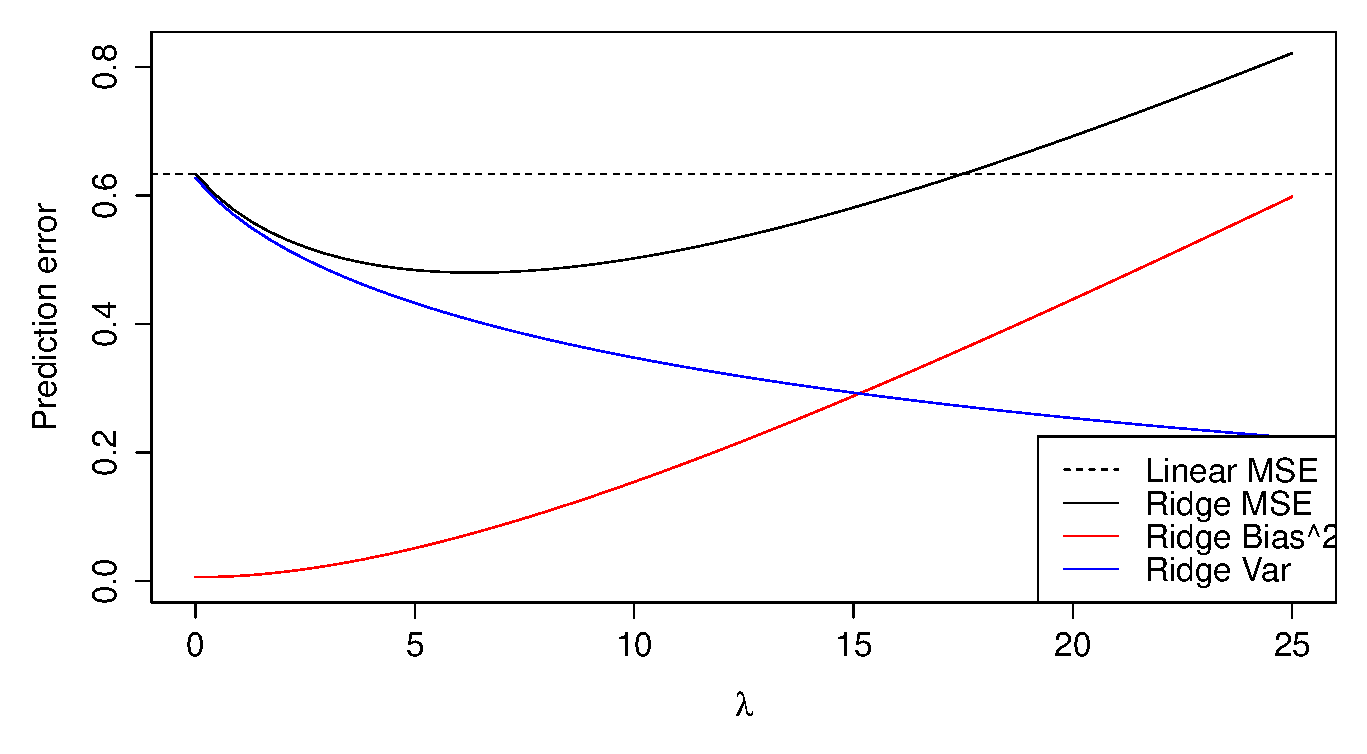
\includegraphics[width=0.8\linewidth]{plots/biasvariance}
\caption{Bias-variance tradeoff}
\label{fig:biasvariance}
\end{figure}

The figure~\ref{fig:biasvariance} shows the bias-variance tradeoff
given by equation~(\ref{eq:prederror}). Ridge regression shows an
increasing bias and a decreasing variance. Despite OLS has zero bias,
its variance is greater than ridge for small values of $\lambda$.
It can be shown that, in terms of prediction error, ridge (black line)
is lower than OLS (dotted line)~\cite{hoerl+kennard1970}.



\subsection{Selection of lambda}

Despite the bias-variance tradeoff provides a conceptual framework for
determining a good model, is not directly useful. Some popular methods
for determine model selection are:

\begin{itemize}
    \item Akaike information criterion (AIC) (Akaike, 1974)
    \item Bootstrap-based selection (Efron and Tibshirani, 1997)
    \item Cross-validation (Stone, 1974)
\end{itemize}

On the other hand, $\lambda$ can also be used to reduce computational time as it
is shown in equation~(\ref{eq:taylor}). Golub (~\cite{golub1965}) suggested that
$\lambda$ be chosen so that:

\[
\frac{\lambda}{\lambda + \delta^2} < 0.1
\]

\noindent where $\delta$ is a lower bound of the smallest non-zero singular
value $\sigma_k$. One approach is to choose the greatest lower bound for
$\delta=\sigma_k$. Hence:

\[
\frac{\lambda}{\lambda + \sigma_k^2} < 0.1
\]

\noindent if we choose $\lambda=\beta \sigma_k^2$ then we get the following
relation:


\[
\frac{\beta \sigma_k^2}{\beta \sigma_k^2 + \sigma_k^2} =
\frac{\beta}{\beta+1} < 0.1 \Rightarrow \beta < \frac{1}{9}  
\]

Experiments done by ~\cite{coleman+sun2010} have shown that $\beta = 0.01$
produces satisfactory results. This means that $\lambda = 0.01 \sigma_k^2$.

However, get $\sigma_k$ imply obtaining first the SVD, which is
computational expensive.

Since the algorithm presented by ~\cite{coleman+sun2010} already compute the QR
factorization of the matrix $\mathbf{A}$ they show a procedure for getting
a $\lambda$ approximation using QR.

\begin{enumerate}
\item Compute QR factorization: $\mathbf{A} = \mathbf{Q_1R_1}$
\item Let $\mathbf{W}$ denote the set of absolute values of the nonzero diagonal
elements of $\mathbf{R_1}$. Let $w_{\text{min}}$ and $w_{\text{max}}$ denote the
smallest and largest elements of $\mathbf{W}$ respectively. Both 
$\lambda_1 = \hat{\beta} w_{\text{min}}^2$
$\lambda_2 = \hat{\beta} \frac{w_{\text{min}}^2}{w_{\text{max}}^2}$ where
$\hat{\beta}=0.00025$ produce satisfactory results.
\item The $\lambda_{\text{QR}}$ approximation is obtained as:
$\lambda_{\text{QR}} = \frac{\lambda_1 + \lambda_2}{2}$  
\end{enumerate}


\section{Online Ridge regression}

Since 
\begin{equation}
\label{eq:notation}
	\mathbf{A} = 
\left[
  \begin{tabular}{c>{$}c<{$}c}
    --- & \mathbf{a}^{\top}_{1} & ---\\
    --- & \mathbf{a}^{\top}_{2} & ---\\
    & \vdots & \\
    --- & \mathbf{a}^{\top}_{m} & ---
  \end{tabular}
\right]
\quad \text{and} \quad
\mathbf{B} =
\left[
  \begin{tabular}{c>{$}c<{$}c}
    --- & \mathbf{b}_{1} & ---\\
    --- & \mathbf{b}_{2} & ---\\
    & \vdots & \\
    --- & \mathbf{b}_{m} & ---
  \end{tabular}
\right]
\
\end{equation}
Equation~(\ref{eq:optsolRR}) can also be written as:

\begin{eqnarray*}
\label{eq:RReapand}
\mathbf{\mathbf{X}}_{\text{ridge}}&=&(\mathbf{A}^\top \mathbf{A}+ \lambda
\mathbb{I})^{-1}\mathbf{A}^\top \mathbf{B} \\
&=& \displaystyle \big (\sum_{t=1}^m
\mathbf{a}_t \mathbf{a}_t  ^\top + \lambda \mathbb{I}\big )^{-1}
\sum_{t=1}^m \mathbf{a}_t \mathbf{b}_t \, .
\end{eqnarray*}

Lets define $\displaystyle\mathbf{S}= \sum_{t=1}^m \mathbf{a}_t
\mathbf{a}_t  ^\top + \lambda \mathbb{I} $ and $\mathbf{W}=
\displaystyle\sum_{t=1}^m \mathbf{a}_t \mathbf{b}_t$, so the
algorithm~\ref{alg:RR} shows the iterative formulation:

\begin{algorithm}[H]
\begin{algorithmic}[1]
\REQUIRE $\,$ \\
$\{\mathbf{a}_1,\dots,\mathbf{a}_{m} \}$: $m$ input vectors \\
$\{\mathbf{b}_1,\dots,\mathbf{b}_{m} \}$: $m$ target vectors \\
$\lambda$: regularization parameter \\
\ENSURE  $\,$ \\
$\{f(\mathbf{a}_1),\dots,f(\mathbf{a}_{m}) \}$: model predictions \\
\STATE Initialize $\mathbf{S}=\lambda \mathbb{I}$
and $\mathbf{W}=0$
\FOR { $t = 1$ to $m$ }
	\STATE read new $\mathbf{a}_t$
	\STATE $\mathbf{X}=\mathbf{S}^{-1}\mathbf{W}$
	\STATE output prediction $f(\mathbf{a}_t) = \mathbf{X}^\top \mathbf{a}_t$
   	\STATE $\mathbf{S} = \mathbf{S} + \mathbf{a}_t \mathbf{a}_t^\top$
   	\STATE Read new $y_t$
    	\STATE $\mathbf{W} = \mathbf{W} + \mathbf{a}_t \mathbf{b}_t$
\ENDFOR
\end{algorithmic}
\caption{Online Ridge Regression}
\label{alg:RR}
\end{algorithm}



\section{The Aggregating Algorithm for Regression}

The AAR, proposed by~\cite{vovk2001}, is an application of the aggregating
algorithm to the problem of regression. The idea is introduce the new input
vector $\mathbf{x}_{m+1}$ to solve the model parameters: 

\begin{equation}
\label{eq:AARexpand}
\mathbf{X}_{aar} = \displaystyle \big (\sum_{t=1}^{m+1}
\mathbf{a}_t \mathbf{a}_t  ^\intercal + \gamma \mathbb{I}\big )^{-1}
\sum_{t=1}^m \mathbf{a}_t \mathbf{b}_t \, .
\end{equation}

If we define $\displaystyle\mathbf{S}= \sum_{t=1}^{m+1} \mathbf{a}_t
\mathbf{a}_t  ^\intercal + \gamma \mathbb{I} $ and $\mathbf{W}=
\displaystyle\sum_{t=1}^m \mathbf{a}_t \mathbf{b}_t$, the
algorithm~\ref{alg:AAR} is slightly different to the algorithm~\ref{alg:RR}, 
which updated matrix $\mathbf{S}$ before making the prediction:

\begin{algorithm}[ht]
\begin{algorithmic}[1]
\REQUIRE $\,$ \\
$\{\mathbf{a}_1,\dots,\mathbf{a}_{m} \}$: $m$ input vectors \\
$\{\mathbf{b}_1,\dots,\mathbf{b}_{m} \}$: $m$ target vectors \\
$\lambda$: regularization parameter \\
\ENSURE  $\,$ \\
$\{f(\mathbf{a}_1),\dots,f(\mathbf{a}_{m}) \}$: model predictions \\
\STATE Initialize $\mathbf{S}=\lambda \mathbb{I}$
and $\mathbf{W}=0$
\FOR { $t = 1$ to $m$ }
	\STATE read new $\mathbf{a}_t$
   	\STATE $\mathbf{S} = \mathbf{S} + \mathbf{a}_t \mathbf{a}_t^\intercal$
	\STATE $\mathbf{X}=\mathbf{S}^{-1}\mathbf{W}$
	\STATE output prediction $f(\mathbf{a}_t) = \mathbf{X}^\intercal \mathbf{a}_t$
   	\STATE Read new $\mathbf{y}_t$
    	\STATE $\mathbf{W} = \mathbf{W} + \mathbf{a}_t \mathbf{b}_t$
\ENDFOR
\end{algorithmic}
\caption{{\em The aggregating algorithm for regression}}
\label{alg:AAR}
\end{algorithm}



\section{Sliding windows AAR method} \label{sec:ORR}


Vector error correction (VEC) models allow studying the joint dynamic
behaviour of a collection of variables which are cointegrated. 

\textbf{Problems}: 

\begin{itemize}
\item VEC parameter estimation method is computationally expensive 
%when the number of past values and observations increases. 
\item VEC model is adjusted to the data in the least-squares sense
\end{itemize}

The objective is to build a new model which admit more error in the square norm and
also be able to obtain VEC parameters faster.  Due to the large amount
of information arriving in financial markets, the model must be
suitable for using in an online fashion.


Due to the amount of information in the Forex market and their high
variability, sometimes old data is useless for forecasting future
values. 

Despite of RR has been a very successful method, they consider all
the available data for making predictions. 
However, some time series show a strong dependence on the latest
information instead of all the data.  The method proposed consists of
a modification of RR considering a sliding window which contains only
the last $L$ samples %and the new input $\mathbf{x}_t$, 
i.e. $\{\mathbf{x}_i\}_{i=t-L+1}^{t-1}$. 

In order to formulate this algorithm we need to define the
following matrices:
 
\[
\mathbf{X}(t) = 
\begin{bmatrix} 
\mathbf{x}_{t-L}^\intercal \\ \vdots \\ \mathbf{x}_t^\intercal
\end{bmatrix} \; , 
{\bf y}(t) = \begin{bmatrix} y_{t-L} \\ \vdots \\ y_t \end{bmatrix} \; .
\]

The optimal solution using a sliding windows is then:

\begin{equation}
\label{eq:optsolSLAAR}
{\bf \phi}(t)_*=({\bf X}(t)^\intercal{\bf X}(t)+\gamma
\mathbb{I})^{-1}{\bf X}(t)^\intercal{\bf y}(t) \, .
\end{equation}

It is worth noticing that the matrix $\mathbf{X}(t+1)$ is slightly
different from $\mathbf{X}(t)$:

\begin{equation} \label{eq:recform}
\mathbf{X}(t+1) = 
\begin{bmatrix} \mathbf{x}_{t-L+1}^\intercal \\ \vdots \\
\mathbf{x}_{t+1}^\intercal
\end{bmatrix} \, .
\end{equation}

Therefore, the matrix $\mathbf{A}=\mathbf{X}(t+1)^\intercal
\mathbf{X}(t+1) $ can be also calculated as:

\begin{eqnarray*}
\mathbf{A}&=&\mathbf{X}(t)^\intercal \mathbf{X}(t) +  \mathbf{x}_{t+1}
\mathbf{x}_{t+1}^\intercal -
\mathbf{x}_{t-L} \mathbf{x}_{t-L}^\intercal \, .
\end{eqnarray*}

Algorithm \ref{alg:SLRR} shows the complete procedure:

%which is very similar
%to AAR (algorithm~\ref{alg:AAR}) except for the calculation of matrix
%$\mathbf{A}$. 


\begin{algorithm}[ht]
\begin{algorithmic}[1]
\REQUIRE $\,$ \\
$\{\mathbf{x}_1,\dots,\mathbf{x}_m \}$: $m$ input vectors \\
$\{y_1,\dots,y_m \}$: $m$ targets \\
$L$: sliding window size ($L<m$) \\
$\gamma$: regularization parameter \\
\ENSURE  $\,$ \\
$\{f(\mathbf{x}_{L+1}),\dots,f(\mathbf{x}_m) \}$: model predictions \\
\STATE Initialize $\mathbf{A}=\displaystyle \sum_{t=1}^L \mathbf{x}_t
\mathbf{x}_t^\intercal + \gamma \mathbb{I}$
and $\mathbf{b}=\displaystyle \sum_{t=1}^Ly_t \mathbf{x}_t$
\FOR { $t = L+1$ to $m$ }
        \STATE read new $\mathbf{x}_t$
        \STATE output prediction $f(\mathbf{x}_t) =  \mathbf{b}^\intercal
\mathbf{A}^{-1}\mathbf{x}_t$
        \STATE $\mathbf{A} = \mathbf{A} + \mathbf{x}_t \mathbf{x}_t^\intercal-
\mathbf{x}_{t-L-1} \mathbf{x}_{t-L-1}^\intercal  $
        \STATE Read new $y_t$
        \STATE $\mathbf{b} = \mathbf{b} + y_t \mathbf{x}_t - y_{t-L-1}\mathbf{x}_{t-L-1}$
\ENDFOR

\end{algorithmic}
\caption{Recursive Ridge Regression}
\label{alg:SLRR}
\end{algorithm}


\section{Model} \label{sec:proposal}

The proposed model is shown in algorithm~(\ref{alg:proposal}) and
takes account the following: 

\begin{itemize}
\item The VEC model matrices are constructed using differences time series
and cointegration factors and vectors from prices time series.
\item As the cointegration factors and vectors don't vary much at every step, they are recalculated every certain amount of time defined as a parameter.
\item The number of cointegration vectors is set as a parameter.
\item The online ridge regression with sliding window algorithm is used to get VEC parameters.
\item In order to avoid the matrix inverse calculation, we use the Sherman
Morrison formula (see section~\ref{sec:sherman}).
\end{itemize}

The following algorithm shows all these steps:

\begin{algorithm}[ht]
\begin{algorithmic}[1]
\REQUIRE $\,$ \\
$\{\mathbf{p}_1,\dots,\mathbf{p}_N \}$: $N$ price vectors \\
%$\{y_1,\dots,y_m \}$: $m$ targets \\
$L$: sliding window size ($L<m$) \\
$\gamma$: regularization parameter \\
$\mu$: cointegration vector update step \\
$r$: number of cointegration vectors \\
$nlag$: number of past values \\
\ENSURE  $\,$ \\
$\{f(\mathbf{x}_{L+1}),\dots,f(\mathbf{x}_m) \}$: model predictions \\
%\STATE Initialize $\mathbf{A}=\gamma \mathbb{I}$
and $\mathbf{b}=0$
\FOR { $t =1$ to $N-L$ }
	\IF {t == 1 \OR \NOT mod(t,$\mu$)}
	\STATE{$jvectors = \text{getJohansen}(r, \{\mathbf{p}_t,\dots,\mathbf{p}_{t+L} \})$}
	\STATE{$[\mathbf{X} \quad \mathbf{Y}] = \text{createMatrix}(jvectors,\{\mathbf{p}_t,\dots,\mathbf{p}_{t+L} \},nlag)$}
	\STATE{$\mathbf{A}=\displaystyle \sum_{t=1}^L \mathbf{x}_t
\mathbf{x}_t^\intercal + \gamma \mathbb{I}$}
	\STATE{$\mathbf{b}=\displaystyle \sum_{t=1}^Ly_t \mathbf{x}_t$}
	\ELSE
        \STATE $[\mathbf{x}_{L} \quad \mathbf{x}_{1}] =
        \text{createVectors}(\mathbf{X},\mathbf{Y},\mathbf{p}_{t+L},nlag)$
        \STATE output prediction $f(\mathbf{x}_t) =  \mathbf{b}^\intercal
\mathbf{A}^{-1}\mathbf{x}_{L}$
        \STATE $\mathbf{A} = \mathbf{A} + \mathbf{x}_{L} \mathbf{x}_{L}^\intercal-
\mathbf{x}_{1} \mathbf{x}_{1}^\intercal  $
        \STATE Read new $y_t$
        \STATE $\mathbf{b} = \mathbf{b} + y_{L} \mathbf{x}_{L} - y_{1}\mathbf{x}_{1}$
        \ENDIF
\ENDFOR

\end{algorithmic}
\caption{Online VEC model}
\label{alg:proposal}
\end{algorithm}

The functions shown in algorithm~(\ref{alg:proposal}) are described
below:
\begin{itemize}
\item $\text{getJohansen}(r, \{\mathbf{p}_t,\dots,\mathbf{p}_{t+L}
\})$ returns the set of $r$ cointegration vectors get them from the las
$L$ prices.
\item
$\text{createMatrix}(jvectors,\{\mathbf{p}_t,\dots,\mathbf{p}_{t+L}
\},nlag)$ returns the matrices that allow to solve the VEC model get
them from the cointegration vectors, the last $L$ prices and the
number of lags. 
\item
$\text{createVectors}(\mathbf{X},\mathbf{Y},\mathbf{p}_{t+L},nlag)$
returns the new input of the VEC model and the data we will remove.
\end{itemize}

The proposal was compared against a modified VEC model. The modifications are:

\begin{itemize}
\item Only a sliding windows of data is used instead of all past data,
which would increase the size of every new input. This was done in order
to compare execution times.
\item Cointegration vectors and factors are calculated every time step.
\item The number of cointegration vectors are determined by the Johansen method.
\end{itemize}

%Although the algorithm~\ref{alg:SLAAR} shows a recursive formulation, it still has
%to compute an inverse matrix at every step. Considering the fact that
%matrix $\mathbf{A}$ is slightly different at every iteration (see
%equation~(\ref{eq:recform}), it is possible to take advantage of this and express
%the inverse matrix of $\mathbf{A}$ in terms of the inverse matrix computed in
%the previous iteration.
%
%At iteration $t+1$ the matrix $\mathbf{A}(t+1)$ to be inverted is: 
%
%\begin{equation} \label{eq:A}
%	\mathbf{A}(t+1)= {\bf X}(t+1)^\intercal{\bf X}(t+1) + \gamma \mathbb{I}\, ,
%\end{equation}
%but,
%
%\begin{equation*}
%{\bf X}(t+1)^\intercal{\bf X}(t+1) = {\bf X}(t)^\intercal{\bf X}(t) + {\bf
%x}_{t+1} {\bf x}_{t+1}^\intercal - {\bf x}_{t-L} {\bf x}_{t-L} ^\intercal \, .
%\end{equation*}
%For convenience, let us define:
%
%\begin{equation*}
%	\mathbf{C}(t) = {\bf x}_{t+1} {\bf x}_{t+1}^\intercal - {\bf x}_{t-L} {\bf
%x}_{t-L} ^\intercal
%\end{equation*}
%now we can rewrite equation~(\ref{eq:A}) as:
%
% \begin{eqnarray*}
% 	\mathbf{A}(t+1) =& {\bf X}(t)^\intercal{\bf X}(t) + \mathbf{C}(t) + \gamma
%\mathbb{I} \nonumber \\
%	\mathbf{A}(t+1) =& \mathbf{A}(t) + \mathbf{C}(t)
% \end{eqnarray*}
%Therefore matrix inverse $\mathbf{A}^{-1}$ can be written as: 
%
%\begin{eqnarray}
%\label{eq:minverse}
%\mathbf{A}(t+1)^{-1} =& \big(\mathbf{A}(t)+ \mathbf{C}(t) \big)^{-1} \nonumber \\
%	=& \big( ( \mathbb{I} + \mathbf{C}(t)\mathbf{A}(t)^{-1})\mathbf{A}(t)
%\big)^{-1} \nonumber \\
%	=& \mathbf{A}(t)^{-1} ( \mathbb{I} +
%\mathbf{C}(t)\mathbf{A}(t)^{-1})^{-1}
%\end{eqnarray}
%Equation~\ref{eq:minverse} shows that the inverse matrix at iteration $t+1$ can be expressed in
%terms of the inverse matrix at iteration $t$, which was previously calculated. Moreover, if the term
%$\mathbf{C}(t)\mathbf{A}(t)^{-1}$ is small, the right hand side of
%equation~(\ref{eq:minverse}) can be approximated using the Taylor expansion for
%matrices:
%
%\begin{equation} \label{eq:taylor}
%	(\mathbb{I} + \Delta)^{-1} = \mathbb{I} - \Delta + \Delta^2 \pm \dots
%\end{equation}
%The inverse approximation shown in equation~(\ref{eq:taylor}) is more accurate
%when more terms of the Taylor expansion are considered.
%In this way, the inverse of the matrix $\mathbf{A}(t+1)$ is avoided and the
%procedure is computationally much less expensive.
%
%
%\subsection{Inverse matrix approximation} \label{sec:matrixinv}
%
%The inverse matrix can be improved by using the approximation used
%in~\cite{obrien1982}. If we obtain $\mathbf{B}$ as the numerical approximation
%of $\mathbf{A}^{-1} \in Mat(n,n)$, we will have:
%
%\begin{equation} \label{eq:m1}
%\mathbf{A}^{-1} = \mathbf{B} + \epsilon \, ,
%\end{equation}
%where $\epsilon$ is a $n \times n$ matrix with the error approximations values.
%This $\epsilon$ matrix can be approximated by premultiplying by $\mathbf{BA}$ in
%equation~(\ref{eq:m1}):
%
%\begin{align} \label{eq:m2}
%& \mathbf{A}^{-1} = \mathbf{B} + \epsilon  \nonumber \\
%& \mathbf{BAA}^{-1} =  \mathbf{BAB} + \mathbf{BA}\epsilon \, ,
%\end{align}
%but $\mathbf{BAA}^{-1}=\mathbf{B}$ and considering that $\mathbf{BA}\epsilon \approx \epsilon$ we can
%obtain an the following expression for $\epsilon$ using equation~(\ref{eq:m2}):
%
%\begin{align} \label{eq:m3}
%\mathbf{B} =  \mathbf{BAB} + \mathbf{BA}\epsilon \nonumber \\
%\epsilon \approx \mathbf{B}-\mathbf{BAB} \, .
%\end{align}
%Replacing expression~\ref{eq:m3} in equation~(\ref{eq:m1}) we have:
%
%\begin{align} \label{eq:m4}
%\mathbf{A}^{-1} \approx \mathbf{B} + \mathbf{B}-\mathbf{BAB} \nonumber \\
%\mathbf{A}^{-1} \approx 2\mathbf{B} - \mathbf{BAB}
%\end{align}
%The equation~(\ref{eq:m4}) allows us to improve the matrix inverse
%approximation.
%
%The algorithm~\ref{alg:SLAAR} includes the recursive model formulation and the
%matrix inverse optimization. 
%
%In order to initialize the algorithm we need to first get matrix $\mathbf{A}$
%and vector $\mathbf{b}$. The exact inverse matrix for $\mathbf{A}$ is
%calculated once using the first $L$ inputs.
%The nexts inverse matrix calculations are done using Taylor approximation and
%they are improved using the method shown in section~\ref{sec:matrixinv}. 
%
%\begin{algorithm}[ht]
%\begin{algorithmic}[1]
%\REQUIRE $\,$ \\
%$\{\mathbf{x}_1,\dots,\mathbf{x}_T \}$: $T$ input vectors \\
%$\{y_1,\dots,y_T \}$: $T$ targets \\
%$L$: sliding window size ($L<T$) \\
%\ENSURE  $\,$ \\
%$\{f(\mathbf{x}_{L+1}),\dots,f(\mathbf{x}_T) \}$: model predictions \\
%\STATE Initialize $\mathbf{A}=\displaystyle \sum_{t=1}^L \mathbf{x}_t
%\mathbf{x}_t^\intercal + \gamma \mathbb{I}$
%and $\mathbf{b}=\displaystyle \sum_{t=1}^Ly_t \mathbf{x}_t$
%\STATE Calculate $\mathbf{A}^{-1}$
%\FOR { $t = L+1$ to $T$ }
%        \STATE read new $\mathbf{x}_t$
%	\STATE $C = \mathbf{x}_t \mathbf{x}_t^\intercal- \mathbf{x}_{t-L-1} \mathbf{x}_{t-L-1}^\intercal$
%	\STATE Update $\mathbf{A} = \mathbf{A} + C$
%	\STATE $\Delta = C A^{-1}$
%	\STATE Taylor approx. $\mathbf{A}^{-1} = \mathbf{A}^{-1} (\mathbb{I} - \Delta + \Delta^2) $
%	\STATE Improve $\mathbf{A}^{-1} = 2\mathbf{A}^{-1} - \mathbf{A}^{-1} \mathbf{A} \mathbf{A}^{-1}$
%        \STATE output prediction $f(\mathbf{x}_t) =  \mathbf{b}^\intercal
%\mathbf{A}^{-1}\mathbf{x}_t$
%        \STATE Read new $y_t$
%        \STATE $\mathbf{b} = \mathbf{b} + y_t \mathbf{x}_t$
%\ENDFOR
%
%\end{algorithmic}
%\caption{Recursive Ridge Regression}
%\label{alg:proposal}
%\end{algorithm}
%





%\section{Online VEC model}

If we want to update the VEC model with new input data
$\mathbf{y}_{T+1}$, we have to add a new row in matrices
$\mathbf{Y,X}$ and $\mathbf{E}$. 

\begin{eqnarray}
\mathbf{Y} &=& 
                \left[ \begin{array}{ccc}
               \quad & \mathbf{\Delta y}_{p+1} & \quad \\ \hline
               \quad & \mathbf{\Delta y}_{p+2} & \quad \\ \hline
               \quad & \vdots & \quad \\ \hline 
               \quad & \mathbf{\Delta y}_T & \quad \\ 
               \quad & \color{red}\mathbf{\Delta y}_{T+1} & \quad 
               \end{array} \right]
             \\
\mathbf{\Phi^*} &=& 
                \left[ \begin{array}{ccc}
               \phi_{p-1}^* \\ 
               \vdots \\ 
               \phi_{1}^* \\
               \alpha \\
                c   
               \end{array} \right]
\\
\mathbf{X} &=& \begin{bmatrix} \label{offX}
   \mathbf{\Delta y}_2 & \dots & \mathbf{\Delta y}_{p-1} &
   \mathbf{\Delta y}_{p} & \beta'\mathbf{y}_{p} & 1\\
   \mathbf{\Delta y}_3 & \dots & \mathbf{\Delta y}_{p} &
   \mathbf{\Delta y}_{p+1} & \beta'\mathbf{y}_{p+1} &1\\
   \vdots &  \ddots & \vdots & \vdots & \vdots & \vdots\\
   \mathbf{\Delta y}_{T-p+1} & \dots & \mathbf{\Delta y}_{T-2} &
   \mathbf{\Delta y}_{T-1} & \beta'\mathbf{y}_{T-1} &1 \\
   \color{red} \mathbf{\Delta y}_{T-p+2} & \dots & \color{red}\mathbf{\Delta y}_{T-1} &
   \color{red}\mathbf{\Delta y}_{T} & \color{red}\beta'\mathbf{y}_{T}
   & \color{red} 1
   \end{bmatrix}
\\
\mathbf{E} &=& \begin{bmatrix}
              \mathbf{\epsilon}_{p+1} \\ \vdots \\ \mathbf{\epsilon}_T
              \\ \color{red}\mathbf{\epsilon}_{T+1}
             \end{bmatrix}
\end{eqnarray}

\section{Foreign Exchange Rate Data} \label{sec:data}

The data used in this article was obtained from Dukascopy historical
bid and ask prices~\cite{dukascopy}. We used currency prices every
minute from the 2nd of January 2012 to the 18th of November 2013,
which were 987454 inputs.

The available currencies pairs were: AUDCAD, AUDCHF, AUDJPY, AUDNZD,
AUDSGD, AUDUSD, CADCHF, CADHKD, CADJPY, CHFJPY, CHFSGD, EURAUD,
EURCAD, EURCHF, EURDKK, EURGBP, EURHKD, EURJPY, EURNOK, EURNZD,
EURPLN, EURSEK, EURSGD, EURTRY, EURUSD, GBPAUD, GBPCAD, GBPCHF,
GBPJPY, GBPNZD, GBPUSD, HKDJPY, NZDCAD, NZDCHF, NZDJPY, NZDUSD,
SGDJPY, USDCAD, USDCHF, USDDKK, USDHKD, USDJPY, USDMXN, USDNOK,
USDPLN, USDRUB, USDSEK, USDSGD, USDTRY, USDZAR, XAGUSD and XAUUSD.



%\section{Experiments} \label{sec:experiments}

In order to determine the parameter for sliding window size $L$  and
the number of lags, we define a set of base currencies:
EURUSD,GBPUSD,USDJPY,USDCHF and add an extra currency of the rest of
currencies available. The base currencies were chosen because they are
the most transacted currencies.

Later, we run VEC model with the 5 currencies considering a variable
window size data (from 100 to 4000) and number of lags (from 1 to 20)
and determine its akaike information criterion (AIC). The figure
~\ref{fig:lagoptimization} shows the zones with AIC levels varying in
color, were white represent the higher values and red represents the
lower values (best models have lower AIC).  We can see that more red
zones are related with high number of lags and windows size around
3000 in 4 examples. The situation is similar in

\begin{figure}[H]
\centering
\begin{tabular}{cc}

\subfloat[Base currencies + AUDSGD]{
    \includegraphics[width=0.4\linewidth]{img/AIC_AUDSGD}
    \label{fig:currency1}
}
&
\subfloat[Base currencies + NZDJPY]{
    \includegraphics[width=0.4\linewidth]{img/AIC_NZDJPY}
    \label{fig:currency2}
}
\\
\subfloat[Base currencies + AUDNZD]{
    \includegraphics[width=0.4\linewidth]{img/AIC_AUDNZD}
    \label{fig:currency3}
}
&
\subfloat[Base currencies + CHFJPY]{
    \includegraphics[width=0.4\linewidth]{img/AIC_CHFJPY}
    \label{fig:currency4}
}

\end{tabular}
\caption{AIC: Lags vs Sliding window size}
\label{fig:lagoptimization}
\end{figure}

 

%\section{\uppercase{Conclusions}}
\label{sec:conclusions}
\noindent A new online vector error correction method was presented. The traditional VECM
was modified in order to use it in an online context. We have shown that our
proposed OVECM considerably reduces execution times without compromising
solution accuracy.  However the execution time of OVECM is only better than
SLVECM if we avoid the cointegration vector calculation using the Johansen
method, this is given by the avg\_error variable which controls how many times
the method is called.  We could see that our algorithm took much less than a
minute at every step. This means that it could also be used with higher
frequency data and would still provide responses before new data arrives. 
In all the presented scenarios, MAPE is still very high and for future
study, it would be interesting to improve the out-of-sample forecast by
considering more explicative variables, optimizing the windows size, the
number of lags or trying new condition to obtain new cointegration vectors.
Since OVECM is an online algorithm which optimizes processing time, it could be
used by investors as an input for strategy robots. Moreover, some technical
analysis methods could be based on its output. 

\chapter{Proofs}
Some useful proofs for the understanding of this thesis.
\section{The pseudo-inverse computed using the compact
singular value decomposition (SVD)} \label{app:pseudoproof}
\begin{equation}
\mathbf{A}^+ = \mathbf{V_1\Sigma_1^{-1}U_1^\top}
\end{equation}

\textbf{Proof}\quad

In the case matrix $\mathbf{A}$ is non singular, its solution is
straight forward:

\begin{equation}
\label{OLSsolution2}
    \mathbf{\mathbf{X}}=\mathbf{A}^{-1}\mathbf{Y}
\end{equation}


Since the problem shown in equation~(\ref{eq:regproblem}) has not
solution, the minimum norm given by equation~(\ref{OLSsolution2}) is
obtained by solving the equivalent problem:

\begin{equation*}
\label{eq:proyectorsol}
\mathbf{A \hat{\mathbf{X}} = PY} 
\end{equation*}


\noindent where $\mathbf{P=U_1 U_1^\top}$ is the projection onto the
Col($\mathbf{A}$). 

Since $\mathbf{V} = [\underset{(n \times k)}{\mathbf{V_1}} |
\underset{(n \times k)}{\mathbf{V_2}}]$ and $\mathbf{V_1^\top V_2 =
0}$ we can express $\mathbf{\hat{\mathbf{X}}} = \mathbf{V_1 \mathbf{X}_1 + V_2 \mathbf{X}_2}$
with $\mathbf{\mathbf{X}_2=0}$ because $\mathbf{\hat{\mathbf{X}}}$ lives in the
$\text{Row}(\mathbf{A})$ given by $\mathbf{V_1}$, so we have:

\begin{eqnarray*}
\mathbf{A \hat{\mathbf{X}}} &=& \mathbf{PY} \\
\mathbf{U_1 \Sigma_1 V_1^\top \hat{\mathbf{X}}} &=& \mathbf{U_1 U_1^\top Y} \\
\mathbf{ V_1^\top \hat{\mathbf{X}}} &=&  \mathbf{\Sigma_1^{-1} U_1^\top Y} \\ 
\mathbf{ V_1^\top V_1 \mathbf{X}_1} &=& \mathbf{\Sigma_1^{-1}
U_1^\top Y} \\
\mathbf{\mathbf{X}_1}&=& \mathbf{\Sigma_1^{-1} U_1^\top Y}
\end{eqnarray*}

\noindent from this result we can obtain $\mathbf{\hat{\mathbf{X}}}$ and
therefore the pseudo-inverse expression:

\begin{eqnarray*}
\mathbf{\hat{\mathbf{X}}} &=& \mathbf{V_1 \mathbf{X}_1} \\
                &=& \mathbf{V_1 \Sigma_1^{-1} U_1^\top Y} \\
\mathbf{A^+} &=& \mathbf{V_1 \Sigma_1^{-1} U_1^\top} \, .
\end{eqnarray*}

$\blacksquare$

\section{Ridge regression optimal solution}\label{app:rroptsection}

\begin{equation*}
\mathbf{\mathbf{X}}_*=(\mathbf{A}^\top \mathbf{A}+\lambda \mathbb{I})^{-1}\mathbf{A}^\top y \, ,
\end{equation*}


\textbf{Proof}\quad

\begin{eqnarray*}
J(\mathbf{\mathbf{X}}) &=&  \| \mathbf{A}\mathbf{\mathbf{X}} - \mathbf{Y} \|_2^2  + \lambda
 \| \mathbf{\mathbf{X}}\| ^2 \\
 &=&  \sum_{t=1}^N (\mathbf{\mathbf{X}}^\top {\bf a}_t-y_t)^2 + \lambda \sum_{i=1}^p \mathbf{X}_i^2 \\
 &=& (\mathbf{X}^\top a_1-y_1)^2 + \dots + (\mathbf{X}^\top a_N-y_N)^2 + \lambda (\mathbf{X}_1^2+\dots+\mathbf{X}_p^2)
\end{eqnarray*}
\noindent taking derivatives
 \begin{eqnarray*}
 \frac{\partial J(\mathbf{\mathbf{X}})}{\partial \mathbf{X}_1}&=& 
 2(\mathbf{X}^\top \mathbf{a}_1-y_1)\mathbf{a}_{11} + \dots + 2(\mathbf{X}^\top \mathbf{a}_N-y_N)\mathbf{a}_{N1} + 2\lambda \mathbf{X}_1 \\
 &=& 2\mathbf{a}_1^\top(\mathbf{A}\mathbf{X}-\mathbf{Y}) + 2\lambda\mathbf{X}_1\\
& \vdots &\\
  \frac{\partial J(\mathbf{\mathbf{X}})}{\partial \mathbf{X}_p}&=& 
 2\mathbf{a}_p^\top(\mathbf{A}\mathbf{X}-\mathbf{Y}) + 2\lambda\mathbf{X}_p 
\end{eqnarray*}

Then we have that:
\begin{eqnarray*}
\frac{\partial J(\mathbf{\mathbf{X}})}{\partial \mathbf{X}}&=& 
 2\mathbf{A}^\top(\mathbf{A}\mathbf{X}-\mathbf{Y}) + 2\lambda\mathbf{X}
\end{eqnarray*}
Since $\frac{\partial J(\mathbf{\mathbf{X}})}{\partial \mathbf{X}}=0$ we have:
\begin{eqnarray*}
2\mathbf{A}^\top(\mathbf{A}\mathbf{X}-\mathbf{Y}) + 2\lambda\mathbf{X}&=&0 \\
\mathbf{A}^\top\mathbf{A}\mathbf{X} - \mathbf{A}^\top\mathbf{Y} + \lambda\mathbf{X} &=& 0\\
(\mathbf{A}^\top\mathbf{A}+\lambda\mathbb{I})\mathbf{X} &=&  \mathbf{A}^\top\mathbf{Y} \\
\mathbf{X} &=& (\mathbf{A}^\top\mathbf{A}+\lambda\mathbb{I})^{-1}  \mathbf{A}^\top\mathbf{Y}
\end{eqnarray*}

$\blacksquare$

\section{Bias and Variance}\label{app:biasandvariance}

The OLS bias can be obtained as:

\begin{eqnarray*}
Bias(\hat{f}(\hat{\mathbf{X}})) &=& E[\hat{\mathbf{X}}] - \mathbf{X} \\
&=& E[ (\mathbf{A}^\top \mathbf{A})^{-1}\mathbf{A}^\top \mathbf{Y}] - \mathbf{X} \\
&=& E[ (\mathbf{A}^\top \mathbf{A})^{-1}\mathbf{A}^\top (\mathbf{AX})] - \mathbf{X}  \\
&=& \mathbf{X}  - \mathbf{X}  \\
&=&  0
\end{eqnarray*}

The Ridge Regression bias can be obtained as:

\begin{eqnarray*}
\mathbf{X}(\lambda) &=&( \mathbf{A}^\top \mathbf{A} + \lambda \mathbb{I})^{-1}\mathbf{A}^\top \mathbf{Y} \\
&=& (\mathbb{I} + \lambda (\mathbf{A}^\top \mathbf{A})^{-1})^{-1} (\mathbf{A}^\top \mathbf{A})^{-1}\mathbf{A}^\top \mathbf{Y} \\
&=&  (\mathbb{I} + \lambda (\mathbf{A}^\top \mathbf{A})^{-1})^{-1}  \hat{\mathbf{X}} \\
&=& \mathbf{W} \hat{\mathbf{X}} 
\end{eqnarray*}

\noindent where $\mathbf{W}  = (\mathbb{I} + \lambda (\mathbf{A}^\top
\mathbf{A})^{-1})^{-1}  $ it is defined for simplicity. Ridge
regression bias is then obtained as:

\begin{eqnarray*}
Bias(\mathbf{X}(\lambda)) &=& E[\mathbf{X}(\lambda)] - \mathbf{X} \\
&=& E[\mathbf{W}\hat{\mathbf{X}}] - \mathbf{X} \\
&=&  \mathbf{W} \mathbf{X} - \mathbf{X} \neq 0 
\end{eqnarray*}


The variance of OLS is:

\begin{equation*}
Var(\hat{\mathbf{X}}) = \sigma^2 (\mathbf{A}^\top \mathbf{A} )^{-1}
\end{equation*}

\noindent and the variance of ridge regression is:

\begin{eqnarray*}
Var(\mathbf{X}(\lambda)) &=& Var(\mathbf{W}\hat{\mathbf{X}}) \\
&=& E[(\mathbf{W}\hat{\mathbf{X}}-E[\mathbf{W}\hat{\mathbf{X}}])(\mathbf{W}\hat{\mathbf{X}}-E[\mathbf{W}\hat{\mathbf{X}}])^\top] \\
&=& \mathbf{W}E[(\hat{\mathbf{X}}-E[\hat{\mathbf{X}}])(\hat{\mathbf{X}}-E[\hat{\mathbf{X}}])^\top] \mathbf{W}^\top \\
&=& \mathbf{W}Var(\hat{\mathbf{X}})\mathbf{W}^\top \\
&=& \sigma^2 \mathbf{W}(\mathbf{A}^\top \mathbf{A} )^{-1}\mathbf{W}^\top
\end{eqnarray*}

\section{Ridge regression shows an
increasing squared bias and a decreasing variance} \label{app:rrbiasvar}

\textbf{Proof}\quad

Since $Bias(\mathbf{X}(\lambda)) \neq 0$ this imply that

\begin{equation*}
Bias(\mathbf{X}(\lambda)) ^2 > 0 
\end{equation*}

\noindent we know that $\mathbf{A}^\top
\mathbf{A}$ has an eigenvalue decomposition $\mathbf{A}^\top
\mathbf{A} = \mathbf{V} \Sigma \mathbf{V}^{-1}$.


\begin{eqnarray*}
Var(\mathbf{X}(\lambda)) &=& \sigma^2 \mathbf{W}(\mathbf{A}^\top \mathbf{A} )^{-1}\mathbf{W}^\top\\
Var(\mathbf{X}(\lambda)) &=& \sigma^2 (\mathbb{I} + \lambda (\mathbf{A}^\top
\mathbf{A})^{-1})^{-1} (\mathbf{A}^\top \mathbf{A} )^{-1}((\mathbb{I} + \lambda (\mathbf{A}^\top
\mathbf{A})^{-1})^{-1} )^\top \\
&=& \sigma^2 (\mathbb{I} + \lambda (\mathbf{V} \Sigma \mathbf{V}^{-1})^{-1} (\mathbf{V} \Sigma \mathbf{V}^{-1})^{-1}((\mathbb{I} + \lambda (\mathbf{V} \Sigma \mathbf{V}^{-1})^{-1})^{-1} )^\top \\
&=& \sigma^2 \mathbf{V} (\mathbb{I} + \lambda \Sigma^{-1})^{-1} \Sigma^{-1} (\mathbb{I} + \lambda \Sigma^{-1})^{-1}  \mathbf{V}^{-1}\\
&=& \sigma^2 \mathbf{V} \mathbf{D}^{-1} \mathbf{V}^{-1}
\end{eqnarray*}

\noindent where $\mathbf{D}^{-1}  = (\mathbb{I} + \lambda \Sigma^{-1})^{-1} \Sigma^{-1} (\mathbb{I} + \lambda \Sigma^{-1})^{-1}$ is a diagonal matrix with coefficients:

\begin{equation*}
d_i = \frac{\sigma_i^{-1}}{(1+\lambda\sigma_i^{-1})^2}
\end{equation*}

$\blacksquare$




\bibliographystyle{IEEEtran}
\bibliography{reference}

\end{document}
